\chapter{PICKING E MODELAGEM DIRETA}
\label{cap2}

A estratégia de otimização do modelo de velocidades é baseada no método de empilhamento Elemento de Reflexão Comum (ERC).
Este método é uma alternativa ao empilhamento convencional no domínio do Ponto Médio Comum (PMC), tem como
objetivo a construção da seção empilhada a partir de um conjunto de seções de afastamento constante e
fornecer parâmetros importantes na construção do macro modelo de velocidades \cite{cre}.

Estes parâmetros são o raio de curvatura $R_{NIP}$ e o ângulo de emergência do raio normal $\beta_0$ dados para
uma frente de onda hipotética (Onda PIN) que se origina sobre o refletor em um ponto chamado de Ponto de Incidência Normal
(PIN) \cite{hubral}. Assim, a estratégia de inversão do modelo de velocidades consiste em, a partir dos parâmetros $R_{NIP}$
e $\beta_0$, encontrar o modelo que localiza as fontes pontuais PIN sobre o refletor em profundidade.
A estratégia que iremos utilizar é baseada na NIP tomografia \cite{niptomo} e na Stereo tomografia \cite{stereo}.

\begin{figure}[H]
\caption{Picking dos tempos de trânsito sobre um refletor da seção empilhada ERC. Os pontos
em amarelo são os pares $t_0$ e $m_0$ escolhidos.}
\begin{center}
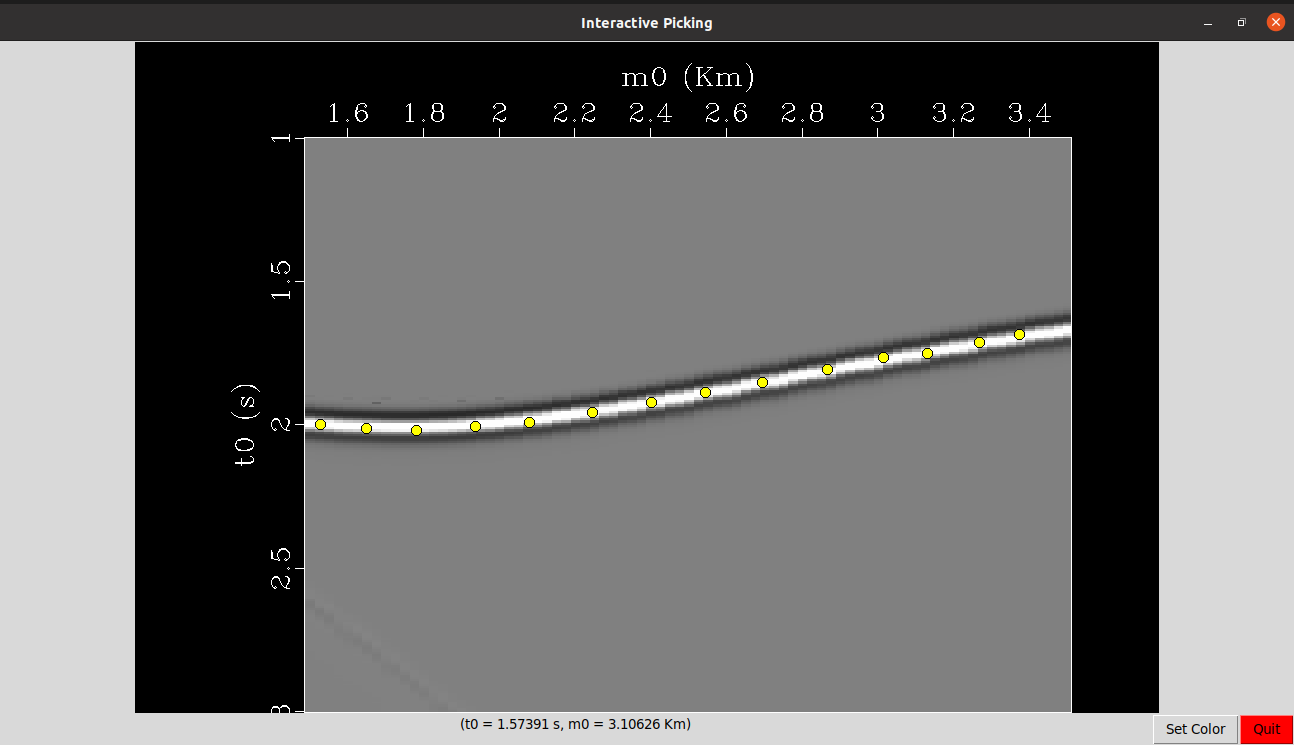
\includegraphics[scale=0.3]{images/picking.png}
\vspace{-0.3cm}
\end{center}
\begin{center}
 Fonte: Do Autor.
\end{center}
\label{fig:2.1}
\end{figure}

Então, após a obtenção da seção empilhada utilizando o empilhamento ERC \cite{relatorio}, realizamos
o picking iterativo dos tempos de trânsito sobre os refletores na seção empilhada ERC (Ver Figura \ref{fig:2.1}).
Estes tempos de trânsito são os tempos duplos $t_0$ dos raios normais que partem da coordenada $m_0$
de um PMC na superfície de aquisição, e incidem normais ao refletor no ponto PIN.

Os tempos de trânsito $t_0$ escolhidos são utilizados para traçar raios normais
a partir da superfície de aquisição em direção ao modelo de velocidades
em profundidade,
de modo a determinar a possível localização do refletor no modelo.
O traçamento continua até que metade do tempo de trânsito $t_0$ seja consumido.
O modelo de velocidades inicial é um modelo de velocidade constante igual à velocidade $v_0$
próxima da superfície de aquisição.

Cada raio normal é iniciado na superfície de aquisição na posição da coordenada $m_0$ e lançado no modelo 
com a direção inicial dada pelo parâmetro $\beta_0$.
O ponto final do raio é a possível localização do refletor em profundidade
e onde será estabelecida a localização das fontes pontuais PIN para o modelo de velocidade
constante. O vetor vagarosidade neste ponto é
normal ao refletor, e com estas informações, o modelo de velocidades inicial é configurado \cite{niptomo}.

\begin{figure}[H]
\caption{Exemplo de traçamento do raio em direção ao modelo de velocidades suavizado.
A partir do traçamento de raios será obtida a localização das fontes PIN em profundidade.}
\begin{center}
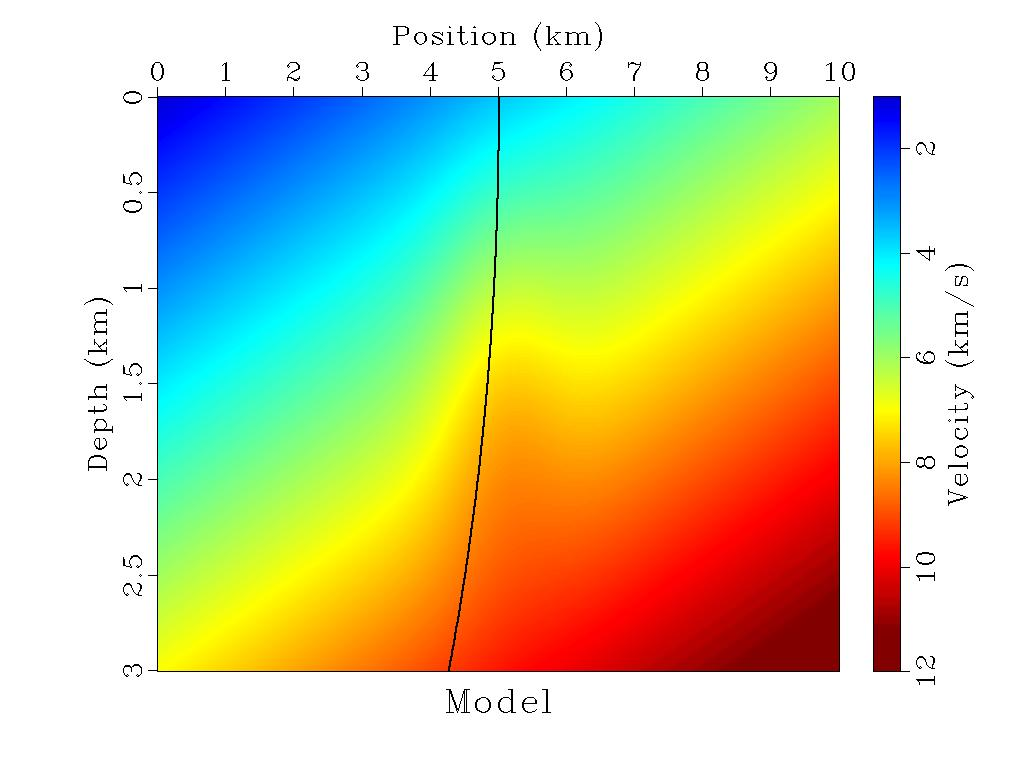
\includegraphics[scale=0.3]{images/raiomodelo.jpg}
\vspace{-0.3cm}
\end{center}
\begin{center}
 Fonte: Do Autor.
\end{center}
\label{fig:2.2}
\end{figure}

Após a determinação das fontes, a modelagem direta é realizada através do traçamento de pares de raios de reflexão
iniciando nas posições das fontes PIN determinadas anteriormente, simulando uma família ERC de raios de reflexão.
Este leque de raios é lançado em direção à superfície de aquisição,
os tempos de trânsito dos raios são armazenados \cite{stereo}.

\begin{figure}[H]
\caption{Exemplo de traçamento de raio a partir de uma fonte pontual em direção a superfície de aquisição.
Os tempos de trânsito do leque de raios é armazenado.}
\begin{center}
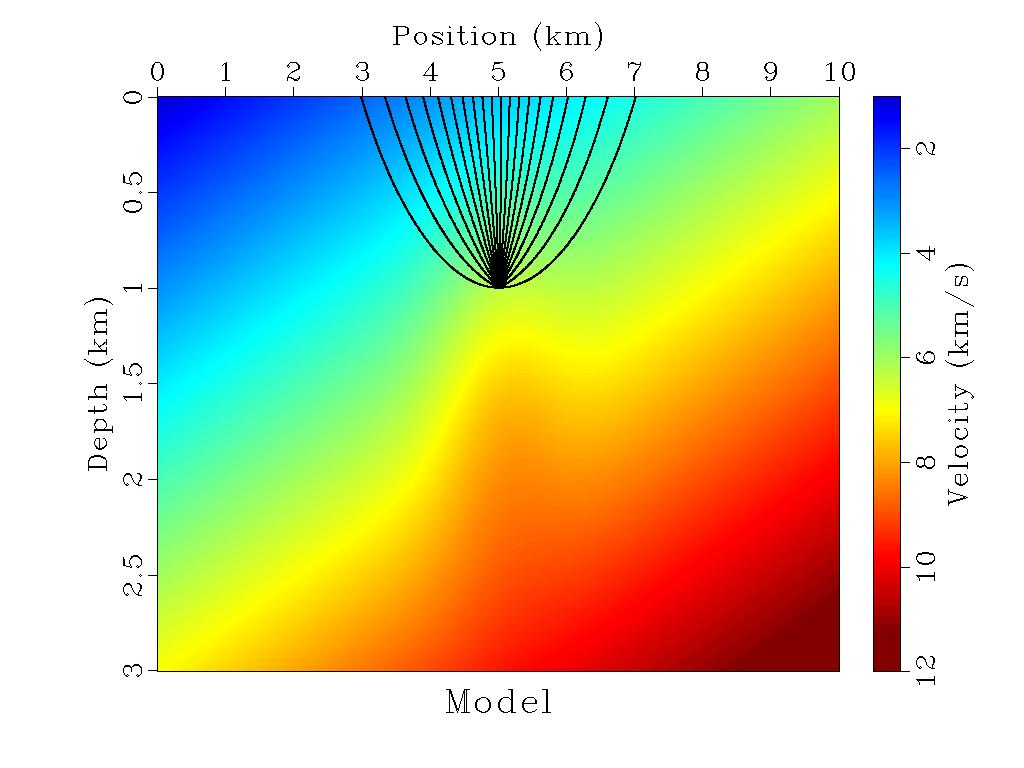
\includegraphics[scale=0.3]{images/raioleque.jpg}
\vspace{-0.3cm}
\end{center}
\begin{center}
 Fonte: Do Autor.
\end{center}
\label{fig:2.3}
\end{figure}

Os tempos de trânsito dos raios de reflexão obtidos no traçamento de raios são comparados com os tempos
de trânsito da aproximação de tempo de trânsito ERC a seguir \cite{cre,relatorio}:

\begin{multline}
\label{eq:2.1}
t(m,h)= \left( \tau_0-\frac{2R_{NIP}}{v_0} \right) 
+\frac{R_{NIP}}{v_0}\sqrt{1-2\alpha(m-m_0+h)+\frac{(m-m_0+h)^2}{R_{NIP}^2}} \\
+\frac{R_{NIP}}{v_0}\sqrt{1+2\alpha(m-m_0-h)+\frac{(m-m_0-h)^2}{R_{NIP}^2}}
\end{multline}

Onde $m$ é a coordenada do PMC, $h$ é a coordenada do afastamento entre fonte e receptor e
$\alpha$ é um parâmetro de assimetria dado em função de $R_{NIP}$ e $\beta_0$.
As diferenças $e_i$ entre os tempos de trânsito do traçamento de raios e dos tempos de trânsito
calculados são somadas segundo a fórmula \cite{stoffa}:

\begin{equation}
\label{eq:2.2}
L_2 = \left[ \sum_{i=1}^{ND} |e_i|^2 \right]^\frac{1}{2}
\end{equation}


Esta estratégia de modelagem direta será utilizada nas etapas de inversão do modelos de velocidades nos
próximos capítulos. A norma dois das diferenças nos tempos de trânsito serão utilizadas como critério de
convergência do modelo de velocidades.

